\subsection*{Das Michelson-Interferometer}
%\begin{figure}[h!]
%	\centering
%	\includegraphics[width=0.7\textwidth]{Interferometer.png}
%	\caption{Versuchsaufbau, der eine nicht interferenzfähige Lichtquelle für Interferenz-Experimente erlaubt}
%	\label{Gluhlampe}
%\end{figure}
%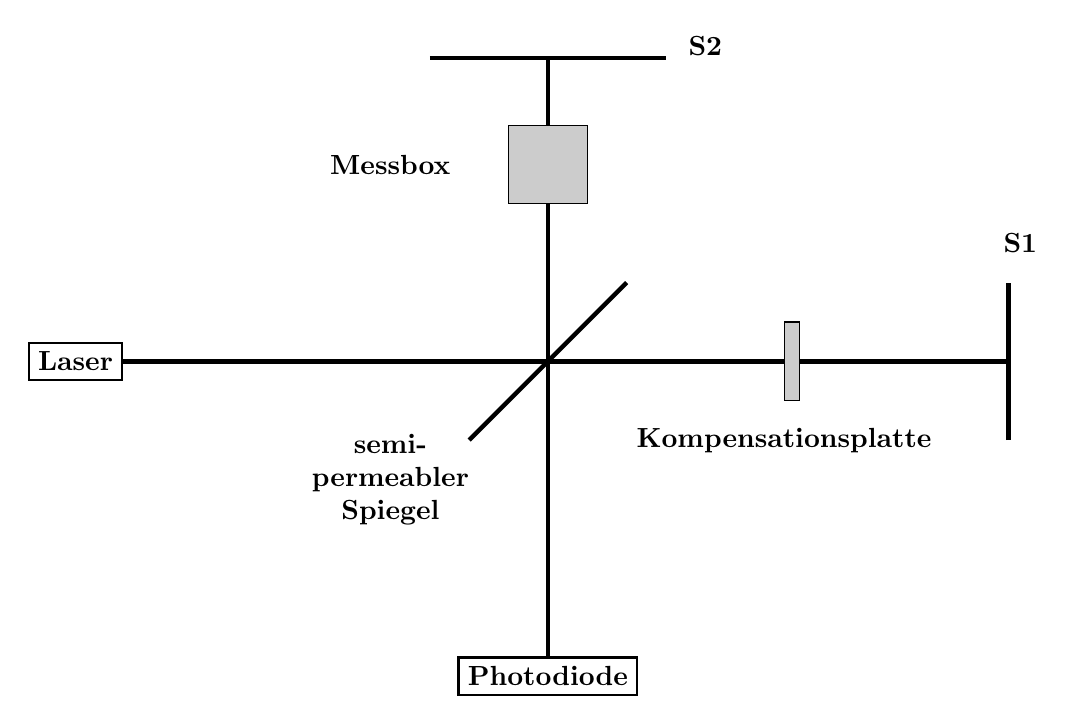
\begin{tikzpicture}
	\node(LASER)at(-6,0)[rectangle,draw,thick]{\textbf{Laser}};
	\node(center)at(0,0){};
	\node(S1)at(6,0){};
	\node(S2)at(0,4){};
	\node(D)at(0,-4)[rectangle,draw,thick]{\textbf{Photodiode}};

%Beschriftung	
	\node(hdl)at(-2,-1.5)[align=center]{\textbf{semi-}\\\textbf{permeabler}\\ \textbf{Spiegel}};
	\node(Box)at(-2,2.5){\textbf{Messbox}};.5
	\node(K)at(3,-1){\textbf{Kompensationsplatte}};
	\node(Spiegel2)at(2,4){\textbf{S2}};
	\node(Spiegel1)at(6,1.5){\textbf{S1}};
	
	\path [-, ultra thick]
	(-1,-1)edge(1,1)            % semipermeabler Spiegel
	(LASER)edge(S1)             % Strahlengang
	(S2)edge(D)                 % Strahlengang
	(-1.5,3.85)edge(1.5,3.85)   % Spiegel 2
	(5.85,-1)edge(5.85,1);      % Spiegel 1
	\filldraw[fill=gray!40!white,draw=black](-0.5,3)rectangle(0.5,2);
	\filldraw[fill=gray!40!white,draw=black](3,0.5)rectangle(3.2,-0.5);
\end{tikzpicture}
Zentraler Bestandteil des Experiments ist ein Michelson-Interferometer (siehe Abbildung VERWEIS). Als Michelson-Interferometer bezeichnet man einen kreuzförmigen Versuchsaufbau, bei dem sich jeweils ein Spiegel (S1) und ein Laser und ein zweiter Spiegel (S2) und ein Photodetektor gegenüber stehen. In der Mitte befindet sich ein semipermeabler Spiegel (SP). \\
Beim Einschalten des Lasers bewegt sich der Lichtstrahl auf SP zu. Dort wird er geteilt. Die beiden einzelnen Strahlen laufen auf S1 oder S2 zu und werden dort reflektiert. Jeder dieser Strahlen wird bei SP abermals geteilt und so treffen zwei parallele Lichtstrahlen auf die Photodiode und erzeugen ein Interferenzbild. Die Intensität im Zentrum wird durch \eqref{Intensitat}
\begin{align}
	I = 2\vec{E}_0^2\left(1+\cos\Delta s\right) \ ,
\end{align}
mit dem Wegunterschied
\begin{align}
	\Delta s = 2(\overline{SPS1}-\overline{SPS2}) \ ,
\end{align}
beschrieben.
\subsection*{Bestimmung der Wellenlänge}
Die Wellenlänge des Lasers (sichtbares Licht) liegt im \si{nm}-Bereich. Um vom Wegunterschied auf die Wellenlänge schließen zu können, muss dieser mit gleicher Genauigkeit bekannt sein. Mit den vorhandenen Mitteln kann das nicht geleistet werden. Alternativ wird ein Aufbau verwendet, bei dem S2 von einem Motor vor und zurück bewegt werden kann. Während der Fahrt wird die Anzahl der Impulse (Intensitätsmaxima) $z$ gezählt. Nach einer Distanz $d >> \lambda$, wird der Motor gestoppt. Innerhalb einer räumlichen Periode $\lambda$ gibt es zwei Impulse, sodass
\begin{align}\label{Wellenlange}
	d = z\frac{\lambda}{2}
\end{align}
gilt.
\subsection*{Bestimmung des Brechungsindex}
Im zweiten Versuchsteil wird die Messbox zwischen SP und S2 benötigt. Die Messbox wird evakuiert, dadurch läuft eines der Strahlenbündel während eines Weges $b$ ein Medium mit Brechungsindex $n' = n_\text{Luft} + \Delta n$. Der Wegunterschied der beiden Strahlen, die an der Photodiode auftreffen ist damit $\Delta n\cdot b$. Lässt man die Luft langsam wieder einströmen, können an der Photodiode Impulse gezählt werden, für die wieder der Zusammenhang \eqref{Wellenlange}
\begin{align}
	\Delta n\cdot b = z \frac{\lambda}{2}
\end{align}
gilt. Da der Brechungsindex im Vakuum $n_0=1$ ist, kann so auf $n_\text{Luft}$ geschlossen werden. \\
Dieser Versuchsteil wird für \ce{CO2} wiederholt, indem die Messbox mit dem Gas gefüllt wird und man es langsam heraus strömen lässt. \\
In diesem zweiten Versuchsteil ist auch die Kompensationsplatte relevant. Sie gleicht die Störungen aus, die durch das Glas an der Messbox verursacht werden.